\documentclass[main]{subfiles}
\usepackage[sols]{workbook}
\numbering{ws3-9}

\begin{document}

\ifSubfilesClassLoaded{%
  \chaptermark{\chapterthree}
}{}

\section{Modeling Interacting Populations} \label{ws3-9}
\begin{framed}
\centerline{\textbf{Lesson Goals}}

You should be able to:
\begin{itemize}
\item Determine and analyze the type of interaction between two species, given a system of first-order differential equations that models their populations
\item Manipulate a system of first-order differential equations to determine how the populations of two species will change in the presence/absence of the other
\item Find the nullclines and equilibrium solutions of a system of first-order differential equations and plot them in the phase plane
\item Use the phase plane to determine the long-term behavior of two interacting populations, given certain initial conditions

\end{itemize}
\end{framed}

\begin{enumerate}

\item 

%\note{Before having students try this problem, I'll give a bit of background on the Lotka-Volterra predator-prey model equations $dx/dt = \alpha x - \beta xy$ and $dy/dt = \gamma x y - \delta y$, and its underlying assumptions:  exponential growth of prey in the absence of the predator, exponential decline of the predator in the absence of prey, and that interactions between predator and prey occur at a rate proportional to the product of their populations.}

Suppose we model the relationship between hyenas and gazelles as follows:


\[ \left\{
\begin{aligned}
\frac{dG}{dt} & = 0.01G - 0.0001 GH = 0.0001G(100- H) \\ 
\frac{dH}{dt} & = -0.1 H + 0.00002 GH = 0.00002(G-5000) H
\end{aligned}
\right.\]
where $G(t)$ gives the number of thousands of gazelles at time $t$. 
where $H(t)$ gives the number of thousands of hyenas at time $t$.
\begin{enumerate}
\item
  \begin{problem}[1in]

    The model above reflects which of the following statements?

  \begin{enumerate}
    \item In the absence of hyenas, the gazelle population grows logistically.
    \item Hyenas are the major predator of gazelles, and in their absence, the gazelle population grows exponentially. 
    \item Hyenas feed on lions, gazelles, and zebra.
    \item Hyenas depend upon gazelles as their primary food source.
    \item Hyenas and gazelles have a competitive relationship.
    \item Hyenas and gazelles have a predator/prey relationship. 
  \end{enumerate}
  \end{problem}

  \begin{solution}
    Let's evaluate these statements one at a time:
    \begin{enumerate}
    \item False.  In the absence of hyenas, gazelles grow exponentially.
    \item True.  If $H = 0$, then $dG/dt = 0.01G$, implying exponential growth of $G$.      
    \item False.  If $G = 0$, then $H$ decays exponentially.  Apparently, $H$ has no alternative food source.
    \item True.
    \item False.  This would mean that {\em both} species would be penalized by the presence of the other.
          Here, $dG/dt$ is reduced in the presence of $H$, but $dH/dt$ increases as $G$ increases.
    \item True.
    \end{enumerate}
  \end{solution}
  

  \item
  \begin{problem}[1in]
  What are the equilibria for this system of differential equations?
  \end{problem}

  \begin{solution}
    Recall that an equilibrium for a system of two differential equations is a pair
    of constant functions (one for each dependent variable) that simultaneously satisfies
    both differential equations.  Because the derivative of a constant function is zero,
    we can seek equilibria by setting both $dG/dt = 0$ and $dH/dt = 0$.  Doing so, we have
    $$ \left\{
      \begin{aligned}   
      0 & = 0.0001G(100- H) \\
      0 & = 0.00002(G-5000) H
      \end{aligned} \right.
    $$
    There are two ways to satisfy the first of these equations:  $G = 0$ or $H = 100$.
    If we choose $G = 0$ then, in order to satisfy the second equation, we would need to
    choose $H = 0$ as well.  In other words, the pair \fbox{$(G,H) = (0,0)$} is an
    equilibrium---it makes sense that if both species are absent, then the populations
    will remain zero forever.  Alternatively, if we choose $H = 100$ then, in order to
    satisfy the second equation, we must choose $G = 5000$.  In other words, the pair
    \fbox{$(G,H) = (5000, 100)$} is also an equilibrium.    
  \end{solution}


  \end{enumerate}

\pspace{\newpage}
%%%%%%%%%%%%%%%%%%%%%%%%%%%%%%%%%%%%%%%%%%%%%%%%%%%%%%%%%%%%%%%%%%%%%%%%%%%%%%%%%%
\item  

  %\note{I'll point out that the predator-prey model can be adapted easily to model either (i) competition between two species for shared resources or (ii) mutualism between two species.  In a competition model, each species' growth rate is inhibited by the presence of the the competing species.  In mutualism, each species' is improved by the presence of the other species.}

    Let $x(t)$ represent the number of hundreds of Xerks at time $t$ and $y(t)$ be
    the number of hundreds of Yowls at time $t$.  For each of the following models, 
    determine the type of interaction between Xerks and Yowls:  competition, 
    predator-prey, or mutualism.  Tell a story that corresponds to each system.

\begin{enumerate}
   \item 
   \begin{problem}[0.1in]   
    $\left\{\begin{aligned}
      \frac{dx}{dt} & = 0.02x  - 0.1xy \\
      \frac{dy}{dt} & = 0.03y -  0.3xy
    \end{aligned}\right.$
   \end{problem}

   \begin{solution}
     The Xerks and the Yowls are in competition, as can be seen by considering
     what happens if precisely one of the species is absent.  If $x = 0$ and $y > 0$,
     then $dy/dt$ is larger than it would have been if $x > 0$, indicating that
     Yowls fare better in the absence of Xerks.  Similarly, Xerks fare better in the
     absence of Yowls.  If one species is absent, then
     the model predicts that the other species would grow exponentially.  Since
     $0.03 > 0.02$, the Yowls can reproduce faster than the Xerks.  
   \end{solution}

\item 
   \begin{problem}[0.1in]   
    $\left\{\begin{aligned}
      \frac{dx}{dt} & = 0.02x\left( 1 - \frac{x}{300} \right) - 0.1xy \\
      \frac{dy}{dt} & = 0.03y\left( 1 - \frac{y}{60}  \right) - 0.3xy
    \end{aligned}\right.$
   \end{problem}

   \begin{solution}
     As in Part (a), the Xerks and the Yowls are in competition, as can be seen by 
     considering what happens if precisely one of the species is absent.  This time,
     if one species is absent, then the other species experiences logistic growth.
     In the absence of Yowls, the environment has a carrying capacity of 300 Xerks.
     In the absence of Xerks, the environment has a carrying capacity of 60 Yowls.
   \end{solution}

\item 
   \begin{problem}[0.1in]   
    $\left\{\begin{aligned}
      \frac{dx}{dt} & = 0.02x  + 0.1xy \\
      \frac{dy}{dt} & = 0.03y +  0.3xy
    \end{aligned}\right.$
   \end{problem}

   \begin{solution}
     The relationship between Xerks and Yowls is mutualistic.  If both
     $x > 0$ and $y > 0$, then {\em both} $dx/dt$ and $dy/dt$ are larger
     than they would be if one of the species were absent.  This model for
     a mutualistic relationship would be very unrealistic---if one species
     were absent, then the other species would experience [unsustainable]
     exponential growth.  The mutualism between the species only enhances
     the growth rates, making the population growth even less sustainable.
   \end{solution}


\item 
   \begin{problem}[0.1in]   
    $\left\{\begin{aligned}
      \frac{dx}{dt} & = -0.02x + 0.1xy \\
      \frac{dy}{dt} & = 0.03y \left( 1 - \frac{y}{5000} \right) -  7xy
    \end{aligned}\right.$
   \end{problem}

   \begin{solution}
      The Xerks and Yowls are engaged in a predator-prey relationship in
      which Xerks are predators and Yowls are prey.  Notice that if Xerks
      are absent (that is if $x = 0$) then $dy/dt$ is larger than it would
      be otherwise.  Similarly, if Yowls are absent then $dx/dt$ is smaller
      than it would be otherwise.  Thus, the Xerks benefit from interactions
      and Yowls are harmed.  The Xerks are fully dependent upon the Yowls
      as food, because if $y = 0$ then the equation $dx/dt = -0.02x$
      predicts exponential decay of Xerks.  In the absence of Xerks, then
      the Yowls obey a logistic growth equation, and the environment's
      carrying capacity for Yowls is 5000.
   \end{solution}

\end{enumerate} 


%%%%%%%%%%%%%%%%%%%%%%%%%%%%%%%%%%%%%%%%%%%%%%%%%%%%%%%%%%%%%%%%%%%%%%%%%%%%%%%%%%
%\pspace{\newpage}
    
\item \label{SIR}

  The Kermack-McKendrick SIR model for spread of an infectious disease works upon
  the following assumptions.  (1) A disease spreads in a community of constant population $N$.
  (2) People are in one of three classes:  (S)usceptible, (I)nfected, or (R)ecovered.
  (3) Susceptible people become infected due to contact with Infected people, at a rate
      proportional to the product of $S$ and $I$.  
  (4) The rate at which Infected individuals transition to Recovered is proportional to the 
      number of infected individuals.  Once recovered, an individual is immune.
  The model equations are
  $$
    \frac{dS}{dt} = -r S I \qquad \frac{dI}{dt} = rSI - \alpha I \qquad \frac{dR}{dt} = \alpha I
  $$
  where $r$ and $\alpha$ are positive constants.

\begin{enumerate}

  \item
  \begin{problem}[0.5in]
    Notice that the equations for $dS/dt$ and $dI/dt$ do not involve $R$, so let's
    focus only on those two equations.  What are the equilibrium solutions?
  \end{problem}

  \begin{solution}
    To have an equilibrium, we need both $dS/dt = 0$ and $dI/dt = 0$.  In order
    for $dS/dt = 0$, we need either $S = 0$ or $I = 0$.  In order for $dI/dt = 0$,
    we need either $I = 0$ or $S = \alpha/r$.  The only way for {\em both}
    $dS/dt = 0$ and $dI/dt = 0$ is if $I = 0$.  This system has \fbox{infinitely
    many equilibria}:  every pair $(S,0)$ is an equilibrium.
    (Practically, we should restrict $0 \leq S \leq N$ for this to make sense, where
    $N$ denotes the total population.)
  \end{solution}

   \item
  \begin{problem}[2in]
    For the Eyam plague of 1666, if time is measured in weeks then data suggests that
    $r = 0.0015$ and $\alpha = 0.45$.  Determine the region of the phase plane in
    which $dI/dt > 0$.  In what region is $dI/dt < 0$?  Suggestion:  Start by finding 
    all points at which $dI/dt = 0$. 
  \end{problem}

  \begin{solution}
    We have $\displaystyle \frac{dI}{dt} = 0.0015 SI - 0.45I \; = \; (0.0015 S - 0.45) I$.
    In order for $dI/dt > 0$, we need both of the factors $(0.0015 S - 0.45)$ and $I$ to be
    positive.  (Remember that negative $I$ makes no sense, because $I$ represents a
    population.)  Thus, in order for $dI/dt > 0$, we need $I > 0$ and $S > 300$.  Similarly,
    we have $dI/dt < 0$ if both $I > 0$ and $S < 300$.

    The interpretation is that if there are enough susceptible people (i.e., more than
    300) to fuel the spread of the disease, then the infection count will get worse before 
    it gets better.
  \end{solution}

  \item
  \begin{problem}[3in]
    %(Exploratory)
    Using the data from Part (b) and initial conditions $S(0) = 493$ and $I(0) = 7$,
    draw your best {\textbf guess} of what the following three graphs would look like:  
    $S(t)$ versus $t$, $I(t)$ versus $t$, and a phase plane trajectory showing 
    $I(t)$ versus $S(t)$.
  \end{problem}

  \begin{solution}
    Since $S(0) = 493$ is larger than 300 and $I(0)$ is positive, from Part (b) we
    know that $dI/dt > 0$.  The number of infected people will increase.  As this happens,
    the number of susceptible people decreases.  Once $S$ dips below 300, then the number
    of infected people will decrease.

    A natural question is:  How many people will catch the disease in the long run?  Will
    everyone?  It turns out that the answer is 'no', but we don't yet have the tools to 
    see why.  The graphs below show what actually happens.  In an upcoming class meeting,
    we'll figure out how to get an exact formula for the curve that the phase plane
    trajectory follows.  Notice that the trajectory strikes the horizontal $S$-axis around
    170.  This means that when the infection runs its course, there were 170 people who
    never caught the disease.

   \begin{center}
     
\includegraphics[width=2.75in]{ws/images/SIR-phase.pdf}
     
\includegraphics[width=2.75in]{ws/images/SIR-traces.pdf}
   \end{center}

  \end{solution}


\end{enumerate}


%%%%%%%%%%%%%%%%%%%%%%%%%%%%%%%%%%%%%%%%%%%%%%%%%%%%%%%%%%%%%%%%%%%%%%%%%%%%%%%%%%
%\pspace{\newpage}
  \item 

\note{This is our introduction to the full process of phase plane analysis. You don't need to get to orienting nullclines, as we'll cover this in the next lesson. But it is helpful to label each nullcline with the derivative that should be equal to 0 there (e.g., labeling the line $H=100$ with $\frac{dG}{dt}=0$), to see more easily how we would orient these nullclines.}

Let's return to our model of the hyena and gazelle population, where $G(t)$ gives the number of thousands of gazelles at time $t$, and $H(t)$ gives the number of thousands of hyenas at time $t$:
\[ \left\{
\begin{aligned}
\frac{dG}{dt} & = 0.01G - 0.0001 GH = 0.0001G(100- H) \\ 
\frac{dH}{dt} & = -0.1 H + 0.00002 GH = 0.00002(G-5000) H
\end{aligned}
\right.\]

\begin{enumerate}

\item
\begin{problem}[2.5in]
Graph the set of all points in the phase plane (with $G$ on the $x$-axis and $H$ on the $y$-axis) for which
        $\frac{dG}{dt} = 0$.  If you do this correctly, you will find that such points fall along
        two distinct lines in this case, and these lines\footnote{In general, nullclines are curves---see
          also \#5.} are known as {\em nullclines}. In this case, we would refer to them as {\em $G$-nullclines}, since $\frac{dG}{dt} = 0$ when we are on these lines.
\end{problem}

\begin{solution}
We begin by setting $\displaystyle \frac{dG}{dt} = 0$, and solving for $G$ and/or $H$. This is best done by using the factored form of $\displaystyle \frac{dG}{dt} = 0$:
\begin{align*}
\frac{dG}{dt} &= 0\\
0.0001G(100- H) &=0\\
G=0 &\text{ or } H=100
\end{align*}

Thus, the $G$-nullclines are $\boxed{G=0}$ and $\boxed{H=100}$. These are graphed in red and labeled on the phase plane below:

\begin{center}
%\resizebox{0.6\textwidth}{!}{
  \begin{tikzpicture}
\begin{axis}[
%axis lines = middle,
            xlabel=$G$,
            ylabel=$H$,
            ytick={100},
            yticklabels={$H=100$},
            ymin=-5,
            xmin=-10,
            xmax=9000,
            ymax=200
            ]   
\addplot[->][red, dashed, domain={0:7000}]{100};
\draw[->, dashed, red] (100,0) to (100,200);
\node at (8000,100) {$\left(\frac{dG}{dt}=0\right)$};
\node at (1700,200) {$G=0~\left(\frac{dG}{dt}=0\right)$};
\end{axis}
\end{tikzpicture}
\end{center}

Notice that we only need to plot the first quadrant of the phase plane, as we can assume that the gazelle and hyena populations are always non-negative.

\end{solution}
       
\item 
\begin{problem}[0.5in]
Plot the $H$-nullclines for this system on the phase plane above -- that is, plot the lines in the phase plane on which $\frac{dH}{dt} = 0$. 
\end{problem}


\begin{solution}
This time, we set $\displaystyle \frac{dH}{dt} = 0$, and solving for $G$ and/or $H$. This is best done by using the factored form of $\displaystyle \frac{dH}{dt} = 0$:
\begin{align*}
\frac{dH}{dt} &= 0\\
0.00002(G-5000) H&=0\\
G=5000 &\text{ or } H=0
\end{align*}

Thus, the $H$-nullclines are $\boxed{H=0}$ and $\boxed{G=5000}$. These are graphed in blue and labeled on the phase plane below:


\begin{center}
%\resizebox{0.6\textwidth}{!}{
  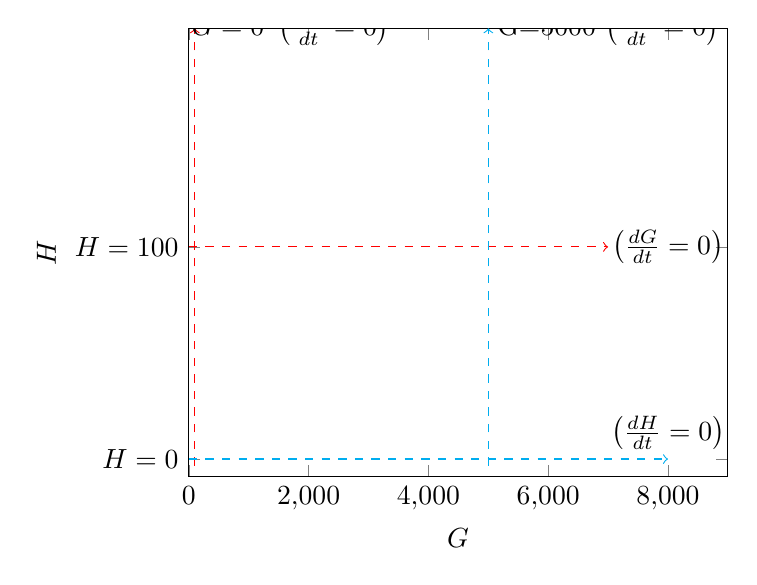
\begin{tikzpicture}
\begin{axis}[
%axis lines = middle,
            xlabel=$G$,
            ylabel=$H$,
            ytick={3,100},
            yticklabels={$H=0$, $H=100$},
            ymin=-5,
            xmin=-10,
            xmax=9000,
            ymax=200
            ]   
\draw[->, red, dashed] (0,100) to (7000,100);
\draw[->, dashed, red] (100,0) to (100,200);
\draw[->, dashed, cyan] (0,3) to (8000,3);
\draw[->, dashed, cyan] (5000,0) to (5000,200);
\node at (8000,100) {$\left(\frac{dG}{dt}=0\right)$};
\node at (8000,15) {$\left(\frac{dH}{dt}=0\right)$};
\node at (1700,200) {$G=0~\left(\frac{dG}{dt}=0\right)$};
\node at (7000,200) {G=5000~$\left(\frac{dH}{dt}=0\right)$};
\end{axis}
\end{tikzpicture}
\end{center}


\end{solution}


\item
\begin{problem}[0.5in]
Find all points in the phase plane above at which both $\frac{dG}{dt} = 0$ and $\frac{dH}{dt} = 0$. We refer to these as {\em equilibrium points}, or {\em equilibria}. What happens if the hyena and gazelle population ever reach these equilibrium levels?
\end{problem}

\begin{solution}
Since the equilibrium points are all the points in the phase plane at which both $\frac{dG}{dt} = 0$ and $\frac{dH}{dt} = 0$, we simply have to look for the intersection points of the $G$-nullclines and the $H$-nullclines. (This is easy to spot, since we've colored the $G$-nullclines and the $H$-nullclines differently.) Thus, the equilibrium points are $\boxed{(0,0)}$ and $\boxed{(5000,100)}$. We have highlighted these points as black dots on the phase plane below.
\begin{center}
%\resizebox{0.6\textwidth}{!}{
  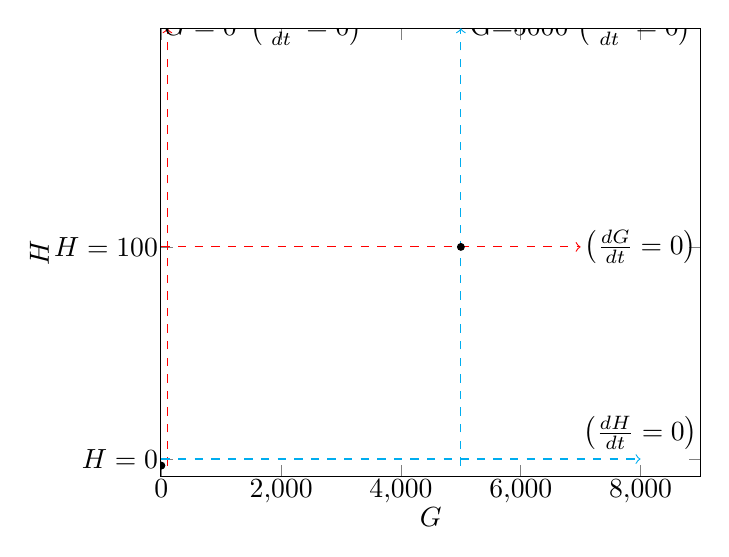
\begin{tikzpicture}[inner sep=0.3mm, vertex/.style={circle,draw,fill=black}]
\begin{axis}[
%axis lines = middle,
            xlabel=$G$,
            ylabel=$H$,
            ytick={3,100},
            yticklabels={$H=0$, $H=100$},
            ymin=-5,
            xmin=-10,
            xmax=9000,
            ymax=200
            ]   
\draw[->, red, dashed] (0,100) to (7000,100);
\draw[->, dashed, red] (100,0) to (100,200);
\draw[->, dashed, cyan] (0,3) to (8000,3);
\draw[->, dashed, cyan] (5000,0) to (5000,200);
\node at (8000,100) {$\left(\frac{dG}{dt}=0\right)$};
\node at (8000,15) {$\left(\frac{dH}{dt}=0\right)$};
\node at (1700,200) {$G=0~\left(\frac{dG}{dt}=0\right)$};
\node at (7000,200) {G=5000~$\left(\frac{dH}{dt}=0\right)$};
\node[vertex] at (5000,100) {};
\node[vertex] at (0,0) {};
\end{axis}
\end{tikzpicture}
\end{center}

If the gazelle and hyena populations ever reached either of these equilibrium levels, they would theoretically remain that way forever, as the rate of change of both populations is 0 at these levels. (This is especially obvious when we are at the equilibrium point $(0,0)$.)

\end{solution}

\item
For each of the initial populations given, plot the trajectory of the hyena and gazelle population on the phase plane above. 
\begin{enumerate}
\item 
\begin{problem}
$G=1000$, $H=0$
\end{problem}

\begin{solution}
If we start at the point $(1000,0)$ on the phase plane, we are on the $G$-axis, which is a $H$-nullcline. Thus, $\frac{dH}{dt}=0$, so there can be no change in $H$, which means there can only be change in the $G$-direction. This tells us that the trajectory can only move left or right from the point $(1000,0)$. 

To determine if the trajectory will go left or right, let's recall that in problem \#1, we determined that the gazelle population would grow exponentially in the absence of hyenas. This would indicate that if we start with $1000$ gazelles and $0$ hyenas, the gazelle population should increase without bound, indicating that our trajectory should move rightward without bound. Thus, we can plot the solution trajectory in the phase plane with purple arrows as follows:

\begin{center}
%\resizebox{0.6\textwidth}{!}{
  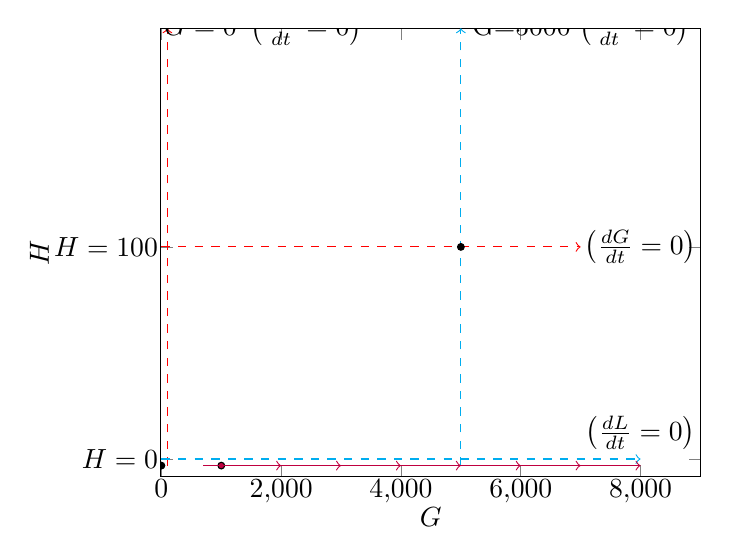
\begin{tikzpicture}[inner sep=0.3mm, vertex/.style={circle,draw,fill=black}, initial/.style={circle,draw,fill=purple}]
\begin{axis}[
%axis lines = middle,
            xlabel=$G$,
            ylabel=$H$,
            ytick={3,100},
            yticklabels={$H=0$, $H=100$},
            ymin=-5,
            xmin=-10,
            xmax=9000,
            ymax=200
            ]   
\draw[->, red, dashed] (0,100) to (7000,100);
\draw[->, dashed, red] (100,0) to (100,200);
\draw[->, dashed, cyan] (0,3) to (8000,3);
\draw[->, dashed, cyan] (5000,0) to (5000,200);
\node at (8000,100) {$\left(\frac{dG}{dt}=0\right)$};
\node at (8000,15) {$\left(\frac{dL}{dt}=0\right)$};
\node at (1700,200) {$G=0~\left(\frac{dG}{dt}=0\right)$};
\node at (7000,200) {G=5000~$\left(\frac{dL}{dt}=0\right)$};
\node[vertex] at (5000,100) {};
\node[vertex] at (0,0) {};

\node[initial] at (1000,0){};
\draw[->, purple] (1000,0) to (2000,0);
\draw[->, purple] (2000,0) to (3000,0);
\draw[->, purple] (3000,0) to (4000,0);
\draw[->, purple] (4000,0) to (5000,0);
\draw[->,purple] (5000,0) to (6000,0);
\draw[->, purple] (6000,0) to (7000,0);
\draw[->, purple] (700,0) to (8000,0);
\end{axis}
\end{tikzpicture}
\end{center}

It is important to note that while the phase plane can tell us the general direction of a trajectory, it \textit{cannot} tell us at what time we will reach a certain point. For example, the phase plane tells us that the gazelle population will eventually hit 1000, but it cannot tell us \textit{when} the population of gazelles will reach 2000. However, in this case, since $G=1000$ and $H=0$ at $t=0$, we'll have the differential equation $\frac{dG}{dt} = 0.01G$, which has a general solution of $G(t)=Ce^{0.01t}$. Using the initial condition, we can solve for $C$ to get the actual solution $G(t)=1000e^{0.01t}$ So we can use this solution to find out exactly when the gazelle population will hit a certain threshold. 

In short, the phase plane only gives us \textit{qualitative} data, while the actual solution function gives us \textit{quantitative} data.

\end{solution}

\item 

\begin{problem}
$G=0$, $H=1000$
\end{problem}

\begin{solution}
If we start at the point $(0,1000)$ on the phase plane, we are on the $H$-axis, which is a $G$-nullcline. Thus, $\frac{dG}{dt}=0$, so there can be no change in $G$, which means there can only be change in the $H$-direction. This tells us that the trajectory can only move up or down from the point $(0,1000)$. 

To determine if the trajectory will go up or down, we recall that in problem \#1, we determined that the hyena population would decay exponentially in the absence of gazelles, as gazelles are their only food source. This would indicate that if we start with $1000$ hyenas and no gazelles, the hyena population should decrease exponentially toward 0, indicating that our trajectory should move downward toward the equilibrium point $(0,0)$. Thus, we can plot the solution trajectory in the phase plane with purple arrows as follows:

\begin{center}
%\resizebox{0.6\textwidth}{!}{
  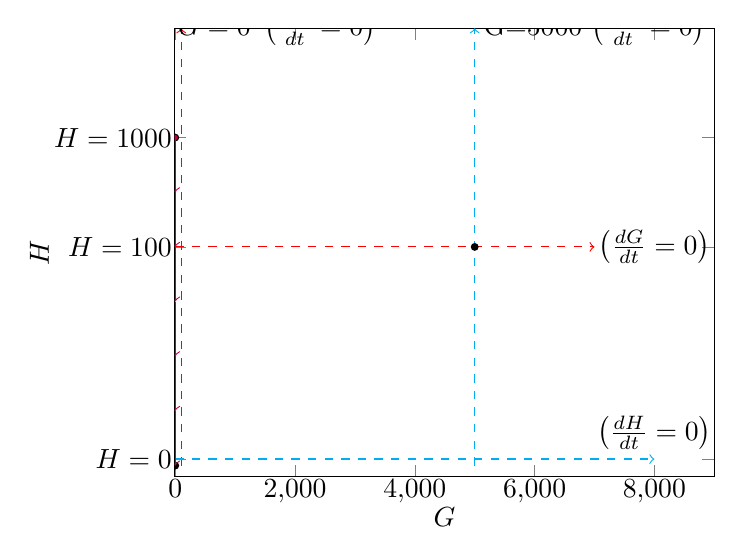
\begin{tikzpicture}[inner sep=0.3mm, vertex/.style={circle,draw,fill=black}, initial/.style={circle,draw,fill=purple}]
\begin{axis}[
%axis lines = middle,
            xlabel=$G$,
            ylabel=$H$,
            ytick={3,100, 150},
            yticklabels={$H=0$, $H=100$, $H=1000$},
            ymin=-5,
            xmin=-10,
            xmax=9000,
            ymax=200
            ]   
\draw[->, red, dashed] (0,100) to (7000,100);
\draw[->, dashed, red] (100,0) to (100,200);
\draw[->, dashed, cyan] (0,3) to (8000,3);
\draw[->, dashed, cyan] (5000,0) to (5000,200);
\node at (8000,100) {$\left(\frac{dG}{dt}=0\right)$};
\node at (8000,15) {$\left(\frac{dH}{dt}=0\right)$};
\node at (1700,200) {$G=0~\left(\frac{dG}{dt}=0\right)$};
\node at (7000,200) {G=5000~$\left(\frac{dH}{dt}=0\right)$};
\node[vertex] at (5000,100) {};
\node[vertex] at (0,0) {};

\node[initial] at (0,150){};
\draw[->, purple] (0,150) to (0,125);
\draw[->, purple] (0,125) to (0,100);
\draw[->, purple] (0,100) to (0,75);
\draw[->, purple] (0,75) to (0,50);
\draw[->,purple] (0,50) to (0,25);
\draw[->,purple] (0,25) to (0,0);
\end{axis}
\end{tikzpicture}
\end{center}

As in the last example, we would need to solve the system of differential equations and find an equation for $H(t)$ in order to determine when the hyena population would die out. If we do, we would have a decreasing exponential function, which cannot be equal to 0 for any time $t$. However, we can determine when the hyena population would be equal to 1, which would give us a good sense of when the population would go extinct. (This highlights another way in which our models are flawed and not perfectly representative of reality.)

\end{solution}



\item $G=5000$, $H=100$

\begin{solution}
We saw in part (c) that the point $(5000,100)$ is an equilibrium point. So, if the population of gazelles starts out at 5000, and the population of hyenas begins at 100, our model predicts that neither population would ever change. Thus, the solutions trajectory for this would be the single point $(5000,100)$, which is a fairly boring trajectory since it doesn't move anywhere! 

This illustrates an important point: \textit{an equilibrium point is always a solution trajectory in and of itself. In other words, an equilibrium point in the phase plane is a solution to the system of differential equations.}

Also, this example highlights yet another way in which our model does not perfectly represent nature. In reality, the gazelle population would not simply stay at exactly 5000 for all time; instead, a few gazelles may be born, while other gazelles would be preyed upon by the existing hyenas. So the gazelle population would likely fluctuate around 5000. Similarly, the hyena population may grow larger than 100, but some may die of hunger due to a lack of available gazelles for the larger amount of hyenas. So the hyena population would also fluctuate around 100. 

We will look more at behavior around an equilibrium solution in the next lesson.

\end{solution}


\end{enumerate}


 \end{enumerate}

\pspace{1in}
 
%%%%%%%%%%%%%%%%%%%%%%%%%%%%%%%%%%%%%%%%%%%%%%%%%%%%%%%%%%%%%%%%%%%%%%%%%%%%%%%%%%%

      
   \item \label{introduce-nullclines}

     \begin{problem}
      Consider the system
      $$
        \left\{
        \begin{aligned}
        \frac{dx}{dt} & = -e^{-x} + y \\
        \frac{dy}{dt} & = y \cos(x) - y^{2}.
        \end{aligned}
        \right.
      $$
      Sketch the $x$-nullclines and the $y$-nullclines.  Then explain why
        this system has infinitely many equilibria.
      \end{problem}

      \begin{solution}
        Setting $dx/dt = 0$ yields one $x$-nullcline:  the graph of $y = e^{-x}$
        is shown in red in the following figure.  There are two $y$-nullclines,
        which may be seen by factoring the right-hand side of the $dy/dt$ equation:
        $$
        \frac{dy}{dt} = y \left[ \cos(x) - y \right].
        $$
        The $y$-nullclines $y = 0$ and $y = \cos(x)$ are shown in blue in the
        following figure.  Because the [red] $x$-nullcline crosses the [blue]
        graph of $y = \cos(x)$ infinitely many times, there are infinitely
        many equilibria.
        \begin{center}
%\resizebox{0.6\textwidth}{!}{
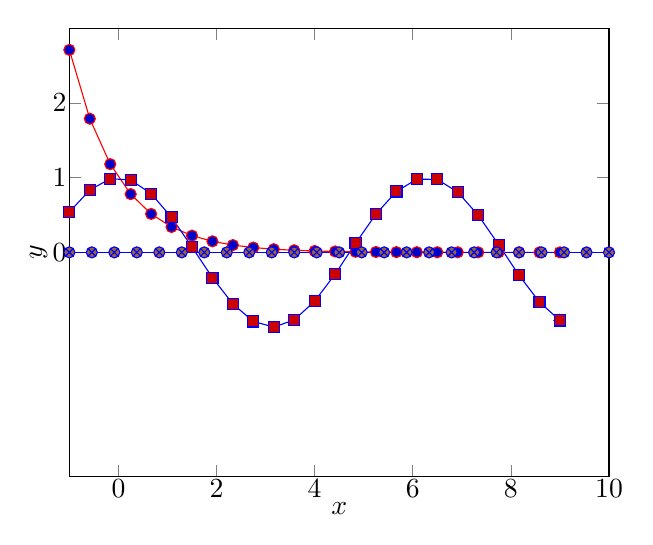
\begin{tikzpicture}[inner sep=0.3mm, vertex/.style={circle,draw,fill=black}, initial/.style={circle,draw,fill=purple}]
\begin{axis}[
%axis lines = middle,
            xlabel=$x$,
            ylabel=$y$,
            ytick={0,1, 2},
            ymin=-3,
            xmin=-1,
            xmax=10,
            ymax=3
            ]   
\addplot+[->, red, domain={-1:9}]{2.71^((-1)*x)};
\addplot+[->, blue, domain={-1:9}]{cos(deg(x))};
\addplot+[->, blue, domain={-1:10}]{0};
\end{axis}
\end{tikzpicture}
\end{center}
      \end{solution}
      
    



    
\end{enumerate}




\end{document}